\documentclass{beamer}
\usepackage[utf8]{inputenc}
\usepackage{graphicx, epsfig}
\usepackage{amsmath,mathrsfs,amsfonts,amssymb}
\usepackage{floatflt}
\usepackage{epic,ecltree}
\usepackage{mathtext}
\usepackage{fancybox}
\usepackage{fancyhdr}
\usepackage{multirow}
\usepackage{enumerate}
\usepackage{epstopdf}
\usepackage{multicol}
\usepackage{algorithm}
\usepackage[noend]{algorithmic}
\usepackage{tikz}
\usepackage{blindtext}
\usetheme{default}%{Singapore}%{Warsaw}%{Warsaw}%{Darmstadt}
\usecolortheme{default}

\setbeamerfont{title}{size=\Huge}
\setbeamertemplate{footline}[page number]{}

\setbeamertemplate{section in toc}[sections numbered]


\makeatletter
\newcommand\HUGE{\@setfontsize\Huge{35}{40}}
\makeatother    

\setbeamerfont{title}{size=\HUGE}
\beamertemplatenavigationsymbolsempty

% latin bold lower
\newcommand{\ba}{\mathbf{a}} 
\newcommand{\bc}{\mathbf{c}} 
\newcommand{\be}{\mathbf{e}} 
\newcommand{\bh}{\mathbf{h}} 
\newcommand{\bp}{\mathbf{p}} 
\newcommand{\bt}{\mathbf{t}} 
\newcommand{\bs}{\mathbf{s}} 
\newcommand{\bu}{\mathbf{u}} 
\newcommand{\bv}{\mathbf{v}} 
\newcommand{\bw}{\mathbf{w}} 
\newcommand{\bx}{\mathbf{x}} 
\newcommand{\by}{\mathbf{y}} 
\newcommand{\bz}{\mathbf{z}} 

% latin bold upper
\newcommand{\bA}{\mathbf{A}} 
\newcommand{\bB}{\mathbf{B}} 
\newcommand{\bC}{\mathbf{C}} 
\newcommand{\bI}{\mathbf{I}} 
\newcommand{\bJ}{\mathbf{J}} 
\newcommand{\bL}{\mathbf{L}} 
\newcommand{\bM}{\mathbf{M}} 
\newcommand{\bP}{\mathbf{P}}
\newcommand{\bQ}{\mathbf{Q}} 
\newcommand{\bR}{\mathbf{R}} 
\newcommand{\bT}{\mathbf{T}} 
\newcommand{\bU}{\mathbf{U}} 
\newcommand{\bV}{\mathbf{V}} 
\newcommand{\bW}{\mathbf{W}} 
\newcommand{\bX}{\mathbf{X}} 
\newcommand{\bY}{\mathbf{Y}} 
\newcommand{\bZ}{\mathbf{Z}} 

% latin cal upper
\newcommand{\cF}{\mathcal{F}} 
\newcommand{\cG}{\mathcal{G}} 
\newcommand{\cI}{\mathcal{I}} 
\newcommand{\cL}{\mathcal{L}} 
\newcommand{\cM}{\mathcal{M}} 
\newcommand{\cN}{\mathcal{N}} 
\newcommand{\cS}{\mathcal{S}} 
\newcommand{\cT}{\mathcal{T}} 
\newcommand{\cW}{\mathcal{W}} 
\newcommand{\cX}{\mathcal{X}} 
\newcommand{\cZ}{\mathcal{Z}} 

% latin bb upper
\newcommand{\bbE}{\mathbb{E}} 
\newcommand{\bbI}{\mathbb{I}} 
\newcommand{\bbP}{\mathbb{P}} 
\newcommand{\bbR}{\mathbb{R}} 

% greek bold lower
\newcommand{\bepsilon}{\boldsymbol{\epsilon}} 
\newcommand{\btheta}{\boldsymbol{\theta}} 
\newcommand{\blambda}{\boldsymbol{\lambda}} 
\newcommand{\bpi}{\boldsymbol{\pi}} 
\newcommand{\bmu}{\boldsymbol{\mu}} 
\newcommand{\bsigma}{\boldsymbol{\sigma}} 
\newcommand{\bphi}{\boldsymbol{\phi}} 

% greek bold upper
\newcommand{\bSigma}{\boldsymbol{\Sigma}} 

\DeclareMathOperator*{\argmin}{arg\,min}
\DeclareMathOperator*{\argmax}{arg\,max}

\newcommand{\createdgmtitle}[1]{\title[\hbox to 56mm{Deep Generative Models  \hfill\insertframenumber\,/\,\inserttotalframenumber}]
	{\vspace{1cm} \\ Deep Generative Models \\ {\Huge Lecture #1}}
	\author{Roman Isachenko}
	\institute{
	Moscow Institute of Physics and Technology
	} 
	\date{2023, Autumn}
}

\usepackage{tikz}
\usetikzlibrary{arrows,shapes,positioning,shadows,trees}

\newcommand\myfootnote[1]{%
  \tikz[remember picture,overlay]
  \draw (current page.south west) +(1in + \oddsidemargin,0.5em)
  node[anchor=south west,inner sep=0pt]{\parbox{\textwidth}{%
      \rlap{\rule{10em}{0.4pt}}\raggedright\scriptsize \textit{#1}}};}

\newcommand\myfootnotewithlink[2]{%
  \tikz[remember picture,overlay]
  \draw (current page.south west) +(1in + \oddsidemargin,0.5em)
  node[anchor=south west,inner sep=0pt]{\parbox{\textwidth}{%
      \rlap{\rule{10em}{0.4pt}}\raggedright\scriptsize\href{#1}{\textit{#2}}}};}
      
\AtBeginSection[]
      {
      	\begin{frame}{Outline}
      		\tableofcontents[currentsection]
      	\end{frame}
      }
      \AtBeginSubsection[]{
      	\begin{frame}{Outline}
      		\tableofcontents[currentsection,currentsubsection]
      	\end{frame}
}
\createdgmtitle{4}

\usepackage{tikz}

\usetikzlibrary{arrows,shapes,positioning,shadows,trees}
%--------------------------------------------------------------------------------
\begin{document}
%--------------------------------------------------------------------------------
\begin{frame}[noframenumbering,plain]
%\thispagestyle{empty}
\titlepage
\end{frame}
%======
\begin{frame}{Recap of previous lecture}
	\vspace{-0.3cm}
	\[
		 \mathcal{L} (\bphi, \btheta)  = \mathbb{E}_{q(\bz | \bx, \bphi)} \left[\log p(\bx | \bz, \btheta) - \log \frac{q(\bz | \bx, \bphi)}{p(\bz)} \right] \rightarrow \max_{\bphi, \btheta}.
	\]	
	\vspace{-0.3cm}
	\begin{block}{M-step: $\nabla_{\btheta} \mathcal{L}(\bphi, \btheta)$, Monte Carlo estimation}
		\vspace{-0.8cm}
		\begin{multline*}
			\nabla_{\btheta} \mathcal{L} (\bphi, \btheta)
			= \int q(\bz|\bx, \bphi) \nabla_{\btheta}\log p(\bx|\bz, \btheta) d \bz \approx  \\
			\approx \nabla_{\btheta}\log p(\bx|\bz^*, \btheta), \quad \bz^* \sim q(\bz|\bx, \bphi).
		\end{multline*}
		\vspace{-0.7cm}
	\end{block}
	\begin{block}{E-step: $\nabla_{\bphi} \mathcal{L}(\bphi, \btheta)$, reparametrization trick}
		\vspace{-0.8cm}
		\begin{multline*}
			\nabla_{\bphi} \mathcal{L} (\bphi, \btheta) = \int r(\bepsilon) \nabla_{\bphi} \log p(\bx | g(\bx, \bepsilon, \bphi), \btheta) d\bepsilon  - \nabla_{\bphi} \text{KL}
			\\ \approx \nabla_{\bphi} \log p(\bx | g(\bx, \bepsilon^*, \bphi), \btheta)  - \nabla_{\bphi} \text{KL}
		\end{multline*}
		\vspace{-0.5cm}
	\end{block}
	\vspace{-0.5cm}
	
	\begin{block}{Variational assumption}
		\vspace{-0.3cm}
		\[
			r(\bepsilon) = \mathcal{N}(0, \bI); \quad  q(\bz| \bx, \bphi) = \mathcal{N} (\bmu_{\bphi}(\bx), \bsigma^2_{\bphi}(\bx)).
		\]
		\[
			\bz = g(\bx, \bepsilon, \bphi) = \bsigma_{\bphi}(\bx) \cdot \bepsilon + \bmu_{\bphi}(\bx).
		\]
	\end{block}
\end{frame}
%=======
\begin{frame}{Recap of previous lecture}
	\begin{block}{Final EM-algorithm}
		\begin{itemize}
			\item pick random sample $\bx_i, i \sim U[1, n]$.
			\item compute the objective:
			\vspace{-0.3cm}
			\[
			\bepsilon^* \sim r(\bepsilon); \quad \bz^* = g(\bx, \bepsilon^*, \bphi);
			\]
			\[
			\cL(\bphi, \btheta) \approx  \log p(\bx | \bz^*, \btheta) - KL(q(\bz^* | \bx, \bphi) || p(\bz^*)).
			\]
			\item compute a stochastic gradients w.r.t. $\bphi$ and $\btheta$
			\begin{align*}
				\nabla_{\bphi} \mathcal{L} (\bphi, \btheta) &\approx \nabla_{\bphi} \log p(\bx | g(\bx, \bepsilon^*, \bphi), \btheta)  - \nabla_{\bphi} \text{KL}(q(\bz | \bx, \bphi) || p(\bz)); \\
				\nabla_{\btheta} \mathcal{L} (\bphi, \btheta) &\approx \nabla_{\btheta} \log p(\bx|\bz^*, \btheta).
			\end{align*}
			\item update $\btheta, \bphi$ according to the selected optimization method (SGD, Adam, RMSProp):
			\begin{align*}
				\bphi &:= \bphi + \eta \nabla_{\bphi} \mathcal{L}(\bphi, \btheta), \\
				\btheta &:= \btheta + \eta \nabla_{\btheta} \mathcal{L}(\bphi, \btheta).
			\end{align*}
		\end{itemize}
	\end{block}
\end{frame}
%=======
\begin{frame}{Recap of previous lecture}
	\begin{minipage}[t]{0.55\columnwidth}
		\begin{block}{Variational autoencoder (VAE)}
		    \begin{itemize}
			    \item VAE learns stochastic mapping between $\bx$-space, from $\pi(\bx)$, and a latent $\bz$-space, with simple distribution. 
			    \item The generative model learns  distribution $p(\bx, \bz | \btheta) = p(\bz) p(\bx |\bz, \btheta)$, with a prior distribution $p(\bz)$, and a stochastic decoder $p(\bx|\bz, \btheta)$. 
			    \item The stochastic encoder $q(\bz|\bx, \bphi)$ (inference model), approximates the true but intractable posterior $p(\bz|\bx, \btheta)$.
		    \end{itemize}
	    \end{block}
	\end{minipage}%
	\begin{minipage}[t]{0.45\columnwidth}
		\vspace{0.7cm}
		\begin{figure}[h]
			\centering
			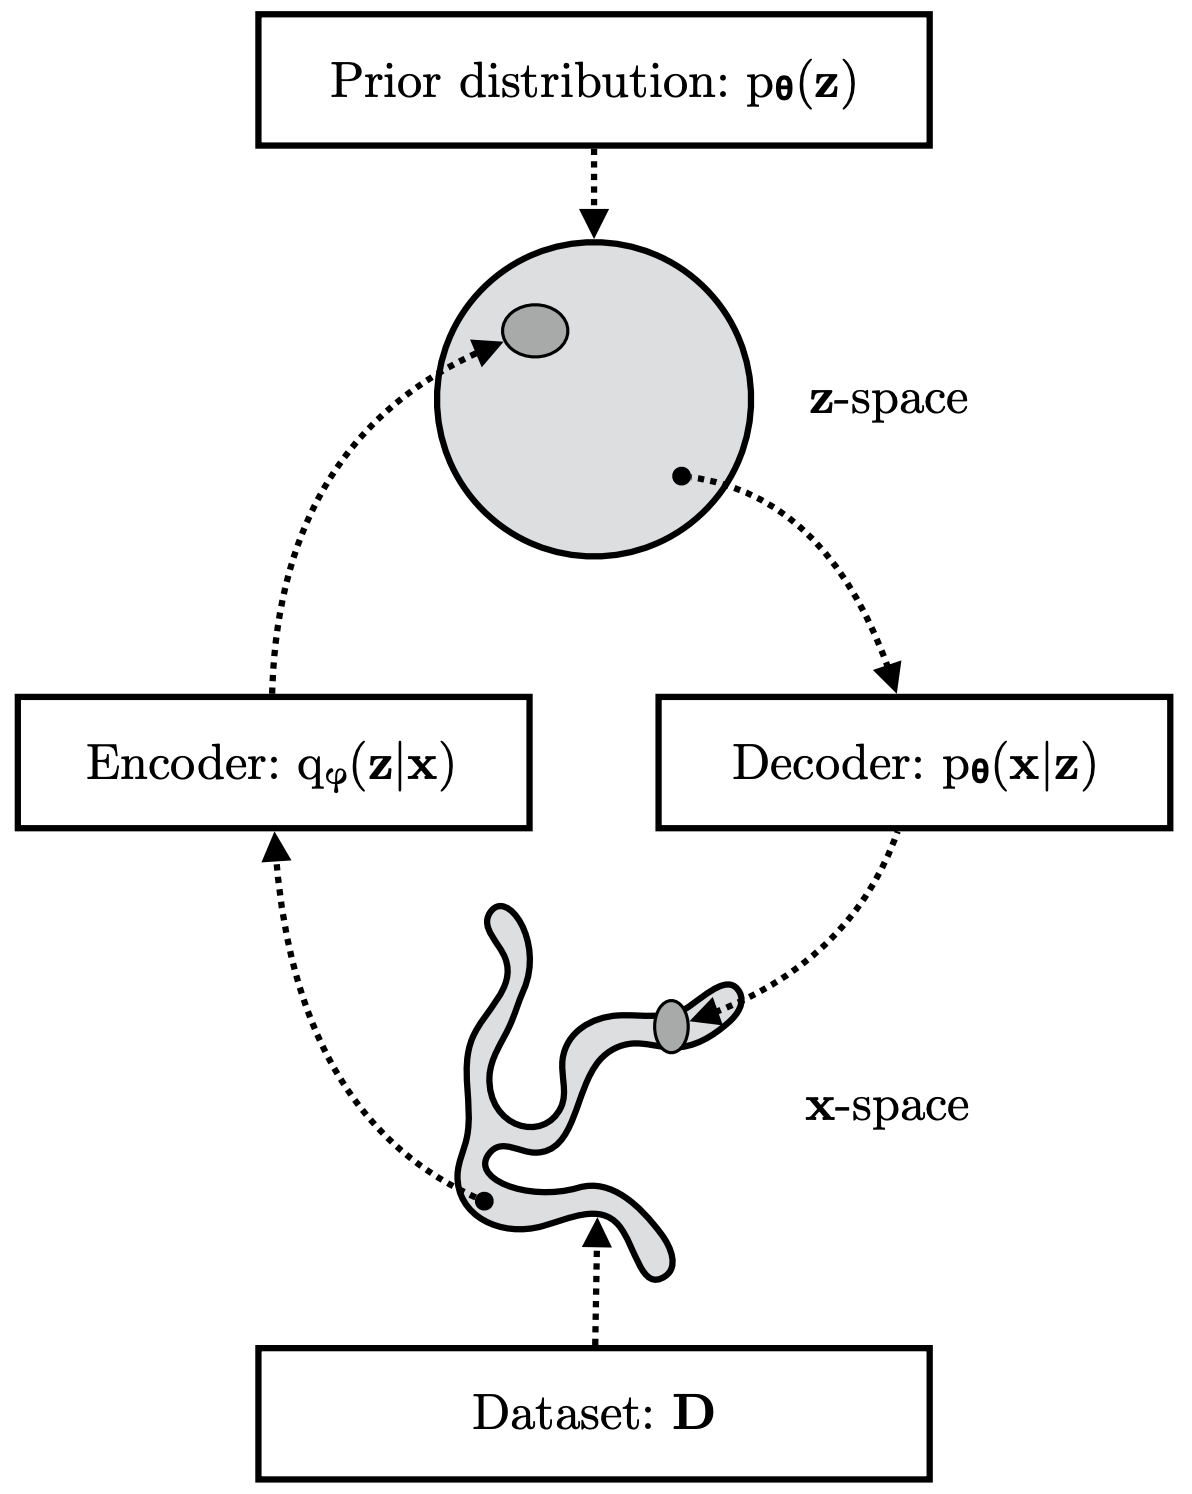
\includegraphics[width=\linewidth]{figs/vae_scheme}
		\end{figure}
	\end{minipage}
	
	\myfootnotewithlink{https://arxiv.org/abs/1906.02691}{Kingma D. P., Welling M. An introduction to variational autoencoders, 2019}
\end{frame}
%=======
\begin{frame}{Recap of previous lecture}
	\begin{block}{VAE objective}
		\vspace{-0.4cm}
		\[
			\log p(\bx | \btheta) \geq \mathcal{L} (q, \btheta)  = \mathbb{E}_{q(\bz | \bx, \bphi)} \log \frac{p(\bx, \bz | \btheta)}{q(\bz| \bx, \bphi)} \rightarrow \max_{q, \btheta}
		\]
		\vspace{-0.5cm}
	\end{block}
	\begin{block}{IWAE objective}
		\vspace{-0.7cm}
		\[
		\mathcal{L}_K (q, \btheta)  = \mathbb{E}_{\bz_1, \dots, \bz_K \sim q(\bz | \bx, \bphi)} \log \left( \frac{1}{K}\sum_{k=1}^K\frac{p(\bx, \bz_k | \btheta)}{q(\bz_k| \bx, \bphi)} \right) \rightarrow \max_{\bphi, \btheta}.
		\]
		\vspace{-0.5cm}
	\end{block}
	\begin{block}{Theorem}
		\begin{enumerate}
			\item $\log p(\bx | \btheta) \geq \mathcal{L}_K (q, \btheta) \geq \mathcal{L}_M (q, \btheta) \geq \mathcal{L} (q, \btheta), \quad \text{for } K \geq M$;
			\item $\log p(\bx | \btheta) = \lim_{K \rightarrow \infty} \mathcal{L}_K (q, \btheta)$ if $\frac{p(\bx, \bz | \btheta)}{q(\bz | \bx, \bphi)}$ is bounded.
		\end{enumerate}
	\end{block}
	\begin{itemize}
		\item IWAE makes the variational bound tighter and extends the class of variational distributions.
		\item Gradient signal becomes really small, training is complicated.
		\item IWAE is a standard quality measure for VAE models.
	\end{itemize}
	\myfootnotewithlink{https://arxiv.org/abs/1509.00519}{Burda Y., Grosse R., Salakhutdinov R. Importance Weighted Autoencoders, 2015}
\end{frame}
%=======
\begin{frame}{Outline}
	\tableofcontents
\end{frame}
%=======
\section{Normalizing flows (NF)}
%=======
\begin{frame}{Likelihood-based models so far...}
	\begin{minipage}[t]{0.5\columnwidth}
		\begin{block}{Autoregressive models}
			\vspace{-0.5cm}
			\[
				p(\bx|\btheta) = \prod_{j=1}^m p(x_j | \bx_{1:j - 1}, \btheta)
			\]
			\vspace{-0.2cm}
			\begin{itemize}
				\item tractable likelihood, 
				\item no inferred latent factors.
			\end{itemize}
		\end{block}
	\end{minipage}%
	\begin{minipage}[t]{0.5\columnwidth}
		\begin{block}{Latent variable models}
			\[
				p(\bx| \btheta) = \int p(\bx, \bz | \btheta) d \bz
			\]
			\begin{itemize}
				\item latent feature representation, 
				\item intractable likelihood.
			\end{itemize}
		\end{block}
	\end{minipage}
	
	\vspace{1cm } 
	How to build model with latent variables and tractable likelihood?
\end{frame}
%=======
\begin{frame}{Generative models zoo}
	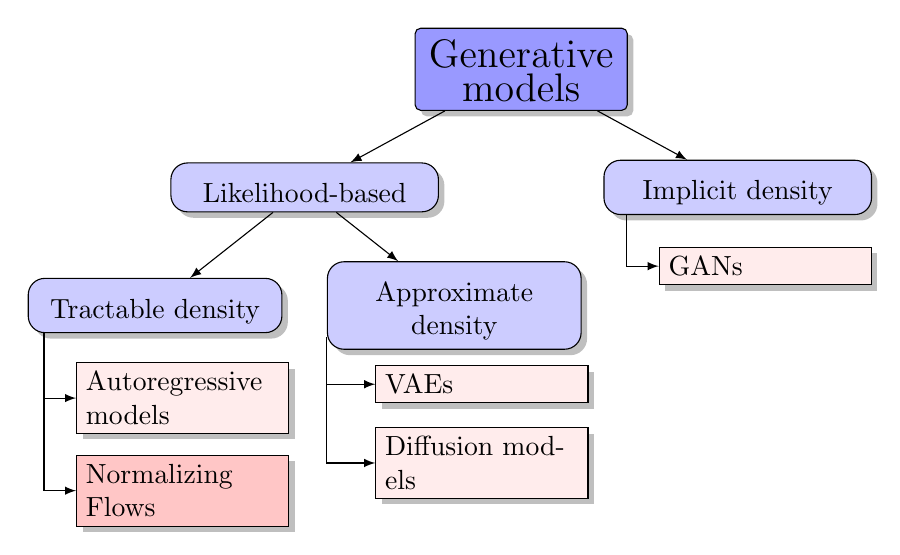
\begin{tikzpicture}[
	 	basic/.style  = {draw, text width=2cm, drop shadow, rectangle},
	 	root/.style   = {basic, rounded corners=2pt, thin, text height=1.1em, text width=7em, align=center, fill=blue!40},
	 	level 1/.style={sibling distance=55mm},
	 	level 2/.style = {basic, rounded corners=6pt, thin, align=center, fill=blue!20, text height=1.1em, text width=9em, sibling distance=38mm},
	 	level 3/.style = {basic, rounded corners=6pt, thin,align=center, fill=blue!20, text width=8.5em},
	 	level 4/.style = {basic, thin, align=left, fill=pink!30, text width=7em},
	 	level 5/.style = {basic, thin, align=left, fill=pink!90, text width=7em},
		edge from parent/.style={->,draw},
		>=latex]
		
		% root of the the initial tree, level 1
		\node[root] {\Large Generative models}
		% The first level, as children of the initial tree
		child {node[level 2] (c1) {Likelihood-based}
			child {node[level 3] (c11) {Tractable density}}
			child {node[level 3] (c12) {Approximate density}}
		}
		child {node[level 2] (c2) {Implicit density}};
		
		% The second level, relatively positioned nodes
		\begin{scope}[every node/.style={level 4}]
		\node [below of = c11, yshift=-5pt, xshift=10pt] (c111) {Autoregressive models};
		
		\node [below of = c12, xshift=10pt] (c121) {VAEs};
		\node [below of = c121] (c122) {Diffusion models};
		\node [below of = c2, xshift=10pt] (c21) {GANs};
		
		\end{scope}
		
		% The second level, relatively positioned nodes
		\begin{scope}[every node/.style={level 5}]
			\node [below of = c111, yshift=-5pt] (c112) {Normalizing Flows};
		\end{scope}
		
		
		% lines from each level 1 node to every one of its "children"
		\foreach \value in {1,2}
		\draw[->] (c11.194) |- (c11\value.west);
		
		\foreach \value in {1,2}
		\draw[->] (c12.194) |- (c12\value.west);
		
		\draw[->] (c2.194) |- (c21.west);
		
	\end{tikzpicture}
\end{frame}
%=======
\begin{frame}{Normalizing flows prerequisites}
	\begin{block}{Jacobian matrix}
		Let $f: \mathbb{R}^m \rightarrow \mathbb{R}^m$ be a differentiable function.
		\[
			\bz = f(\bx), \quad 
			\bJ =  \frac{\partial \bz}{\partial \bx} =
			\begin{pmatrix}
				\frac{\partial z_1}{\partial x_1} & \dots & \frac{\partial z_1}{\partial x_m} \\
				\dots & \dots & \dots \\ 
				\frac{\partial z_m}{\partial x_1} & \dots & \frac{\partial z_m}{\partial x_m}
			\end{pmatrix} \in \bbR^{m \times m}
		\]
		\vspace{-0.3cm}
	\end{block}
	\begin{block}{Change of variable theorem (CoV)}
		Let $\bx$ be a random variable with density function $p(\bx)$ and $f: \mathbb{R}^m \rightarrow \mathbb{R}^m$ is a differentiable, \textbf{invertible} function (diffeomorphism). If $\bz = f(\bx)$, $\bx = f^{-1}(\bz) = g(\bz)$, then
		\begin{align*}
			p(\bx) &= p(\bz) |\det(\bJ_f)| = p(\bz) \left|\det \left(  \frac{\partial \bz}{\partial \bx} \right) \right| = p(f(\bx)) \left|\det \left(  \frac{\partial f(\bx)}{\partial \bx} \right) \right| \\
			p(\bz) &= p(\bx) |\det(\bJ_g)|= p(\bx) \left|\det \left(  \frac{\partial \bx}{\partial \bz} \right) \right| = p(g(\bz)) \left|\det \left(  \frac{\partial g(\bz)}{\partial \bz} \right) \right|.
		\end{align*}
		\vspace{-0.5cm}
	\end{block}
\end{frame}
%=======
\begin{frame}{Jacobian determinant}
	\begin{block}{Inverse function theorem}
		If function $f$ is invertible and Jacobian matrix is continuous and non-singular, then
		\vspace{-0.3cm}
		\[
		\bJ_f = \bJ_{g^{-1}} = \bJ_g^{-1}; \quad |\det (\bJ_f)| = \frac{1}{|\det (\bJ_g)|}.
		\]
		\vspace{-0.3cm}
	\end{block}
	\begin{minipage}{0.55\columnwidth}
		\begin{itemize}
			\item $\bx$ and $\bz$ have the same dimensionality ($\bbR^m$).
			\vfill
			\item $f(\bx, \btheta)$ could be parametric function.
			\vfill
			\item Determinant  of Jacobian matrix $\mathbf{J} =\frac{\partial f(\bx, \btheta)}{\partial \bx}$ shows how the volume changes under the transformation.
		\end{itemize}
	\end{minipage}%
	\begin{minipage}{0.45\columnwidth}
		\begin{figure}
			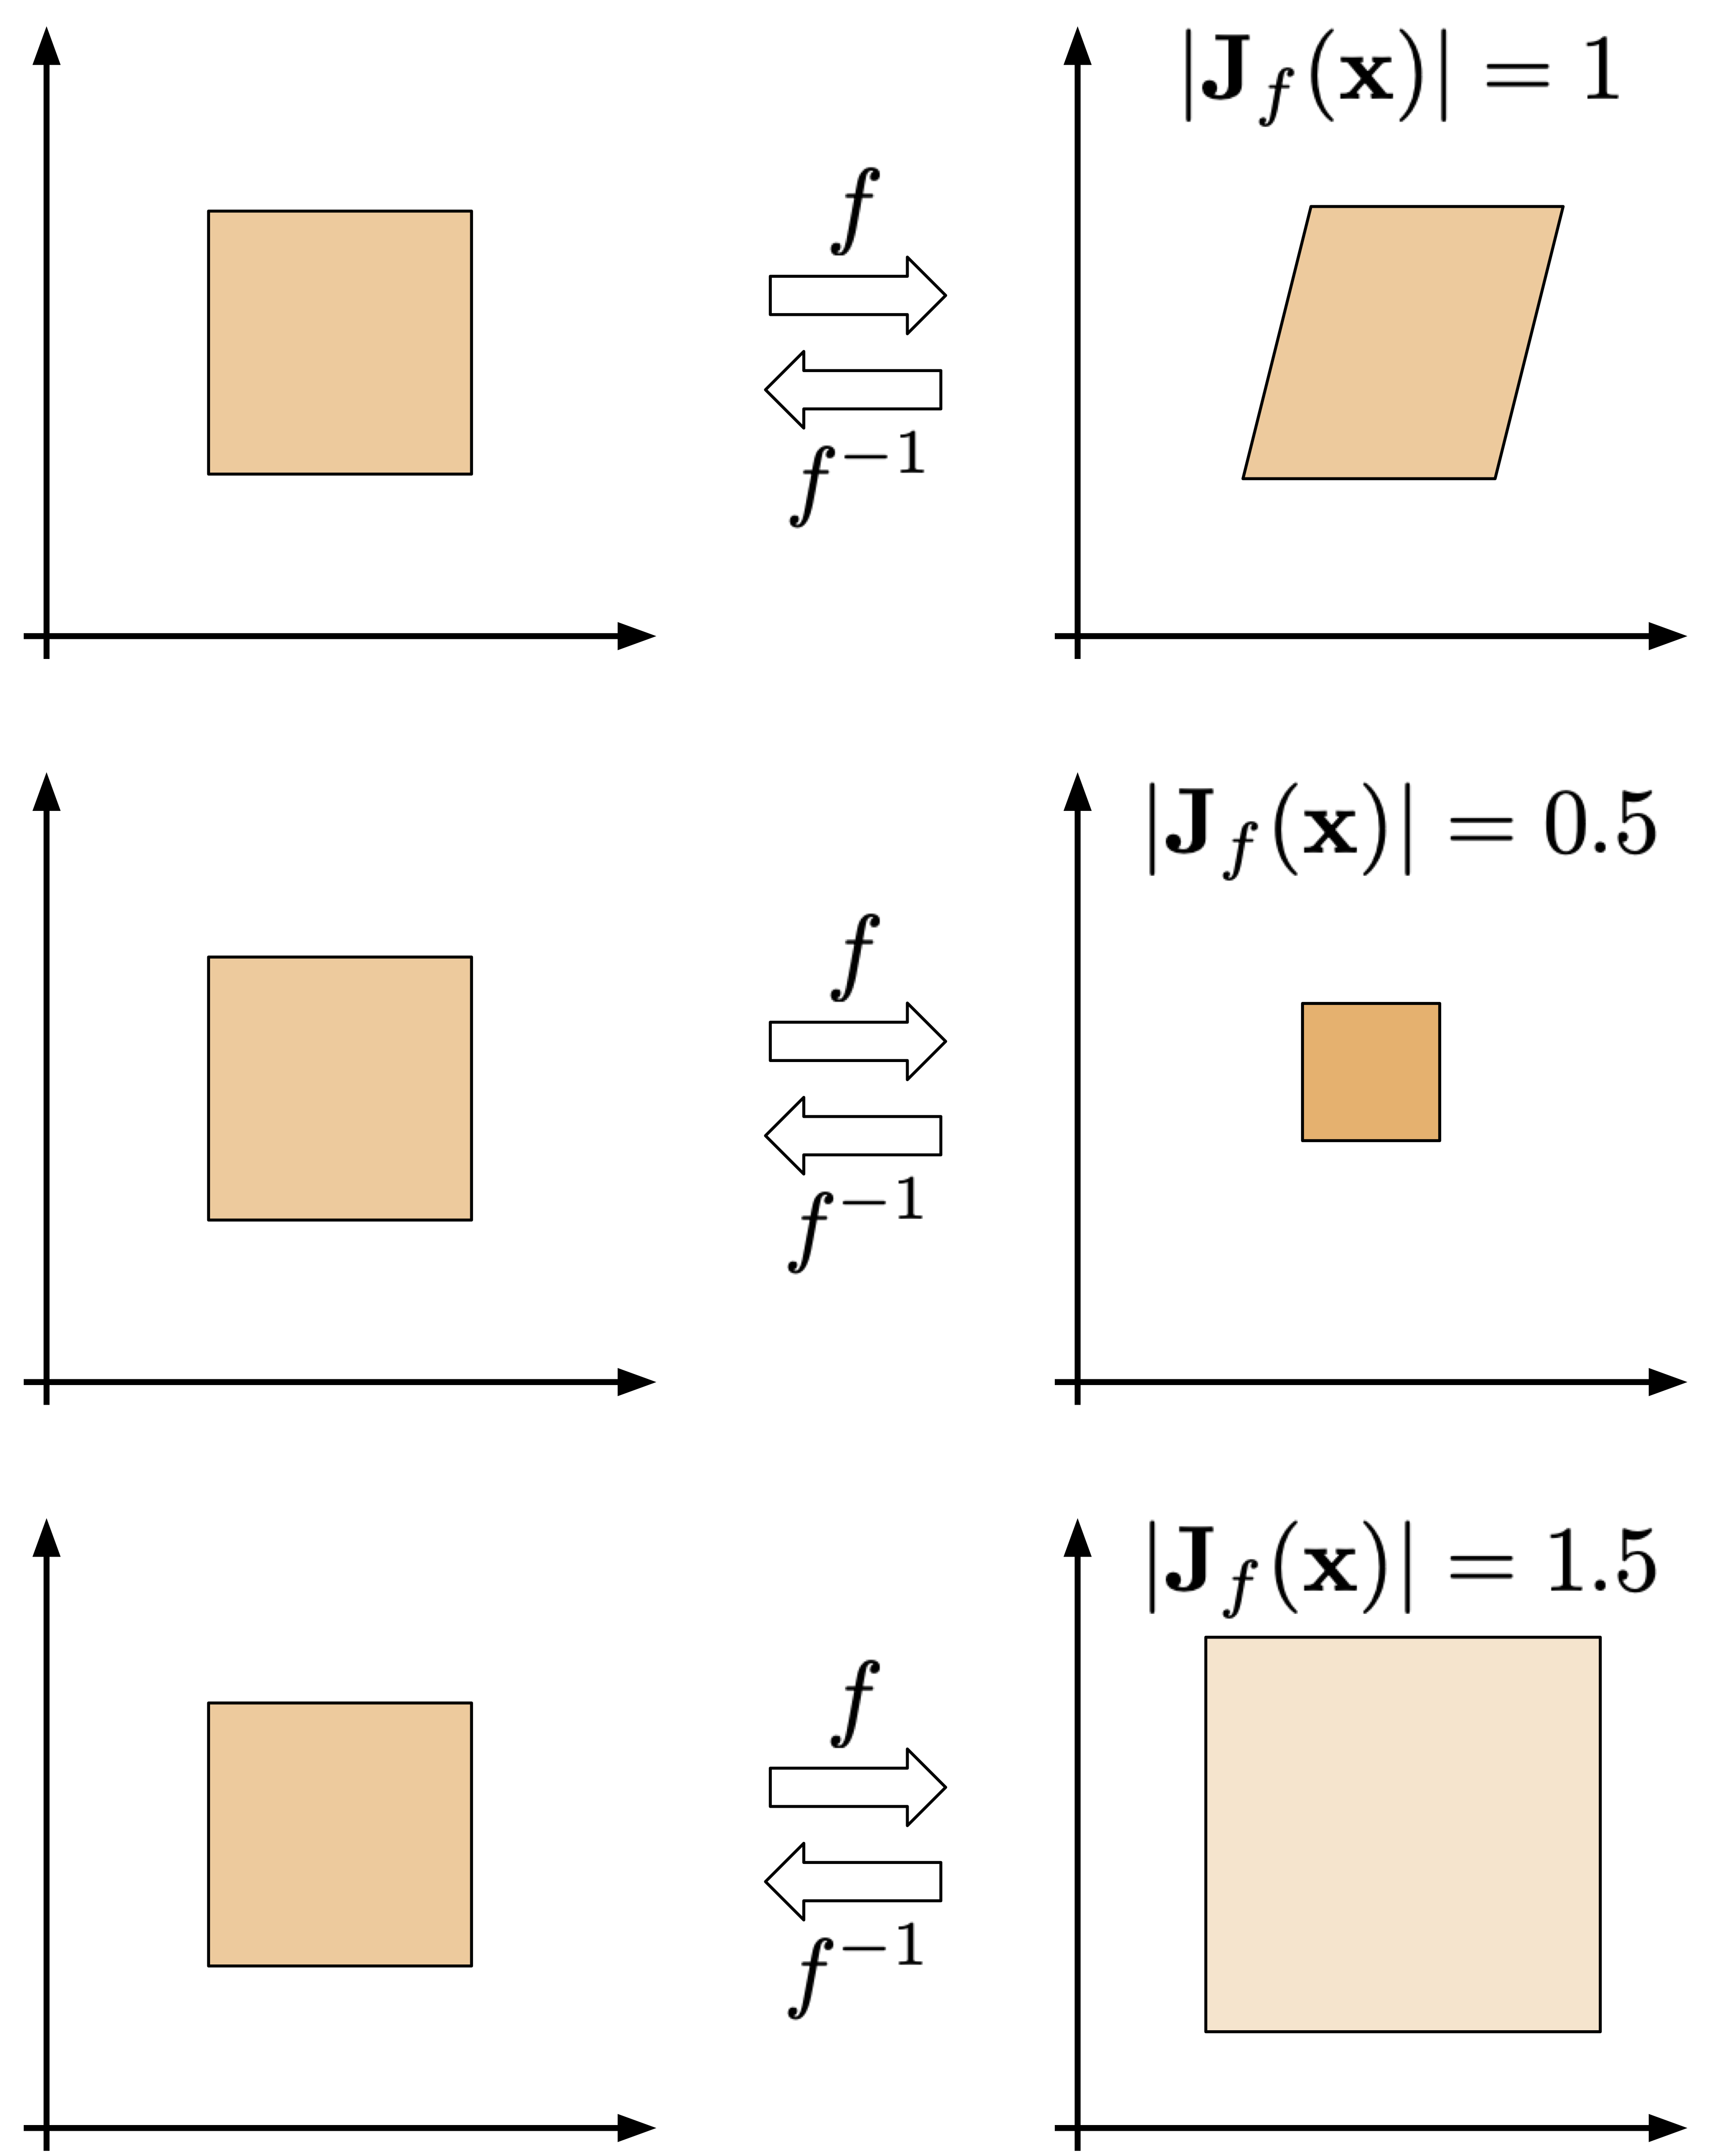
\includegraphics[width=0.8\linewidth]{figs/jacobian_det}
		\end{figure}
	\end{minipage}
	\myfootnotewithlink{https://jmtomczak.github.io/blog/3/3\_flows.html}{https://jmtomczak.github.io/blog/3/3\_flows.html}
\end{frame}
%=======
\begin{frame}{Fitting normalizing flows}
	\begin{block}{MLE problem}
		\vspace{-0.3cm}
		\[
		p(\bx|\btheta) = p(\bz) \left|\det \left(  \frac{\partial \bz}{\partial \bx} \right) \right|  = p(f(\bx, \btheta)) \left|\det \left( \frac{\partial f(\bx, \btheta)}{\partial \bx} \right) \right|
		\]
		\[
		\log p(\bx|\btheta) = \log p(f(\bx, \btheta)) + \log  |\det (\bJ_f) | \rightarrow \max_{\btheta}
		\]
	\end{block}
	\vspace{-0.2cm}
	\begin{figure}
		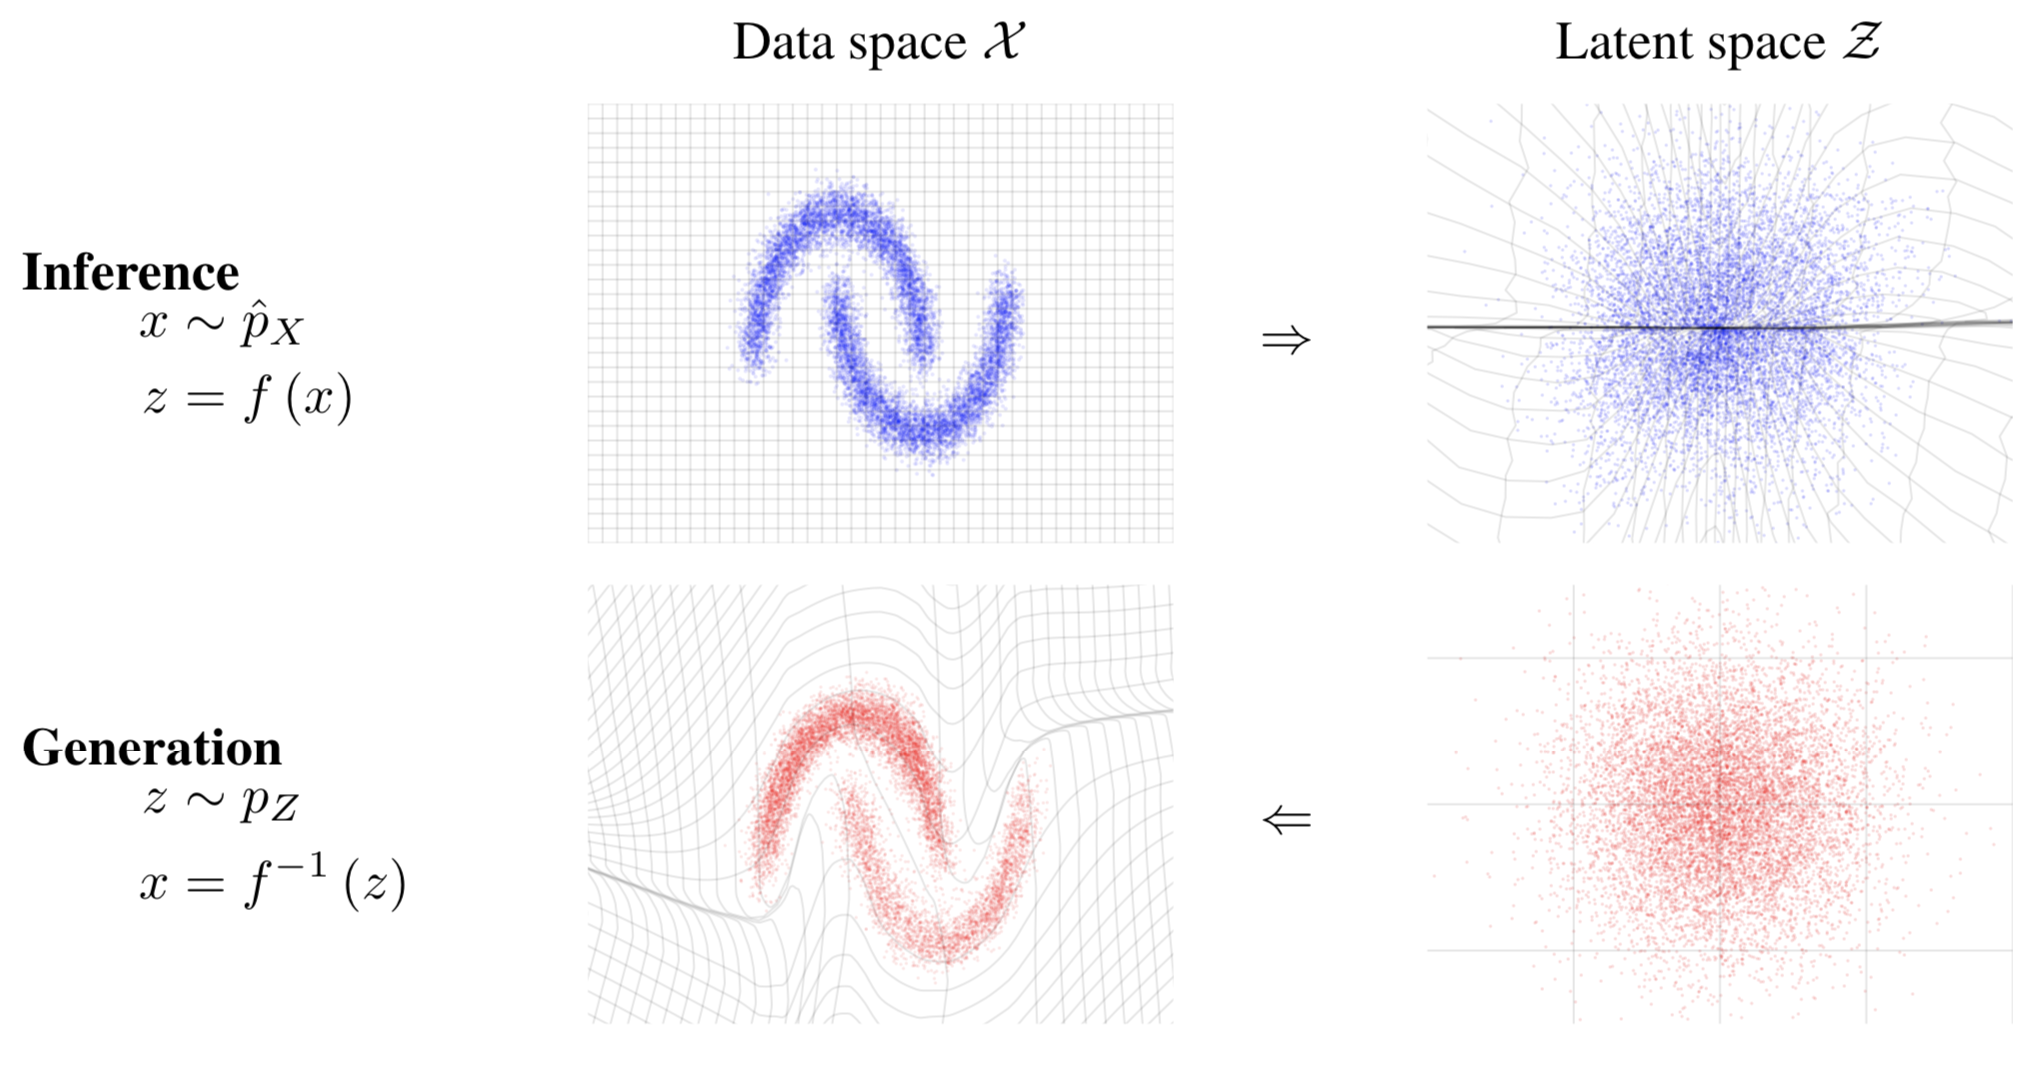
\includegraphics[width=0.85\linewidth]{figs/flows_how2}
	\end{figure}
	\myfootnotewithlink{https://arxiv.org/abs/1605.08803}{Dinh L., Sohl-Dickstein J., Bengio S. Density estimation using Real NVP, 2016} 
\end{frame}
%=======
\begin{frame}{Composition of normalizing flows}
	\begin{block}{Theorem}
		Diffeomorphisms are \textbf{composable} (If $\{f_k\}_{k=1}^K$ satisfy conditions of the change of variable theorem, then $\bz = f(\bx) = f_K \circ \dots \circ f_1(\bx)$ also satisfies it).
	\end{block}
	\vspace{-0.5cm}
	{ \footnotesize
		\begin{multline*}
			p(\bx) = p(f(\bx)) \left|\det \left(\frac{\partial f(\bx)}{\partial \bx} \right) \right| =
			p(f(\bx)) \left|\det \left(\frac{\partial \textbf{f}_K}{\partial \textbf{f}_{K-1}} \dots \frac{\partial \textbf{f}_1}{\partial \bx} \right) \right| = \\ = p(f(\bx)) \prod_{k=1}^K \left|\det \left(\frac{\partial \textbf{f}_{k}}{\partial \textbf{f}_{k-1}} \right) \right|
			= p(f(\bx)) \prod_{k=1}^K |\det ( \bJ_{f_k}) |
		\end{multline*}
	}
	\vspace{-0.3cm}
	\begin{figure}
		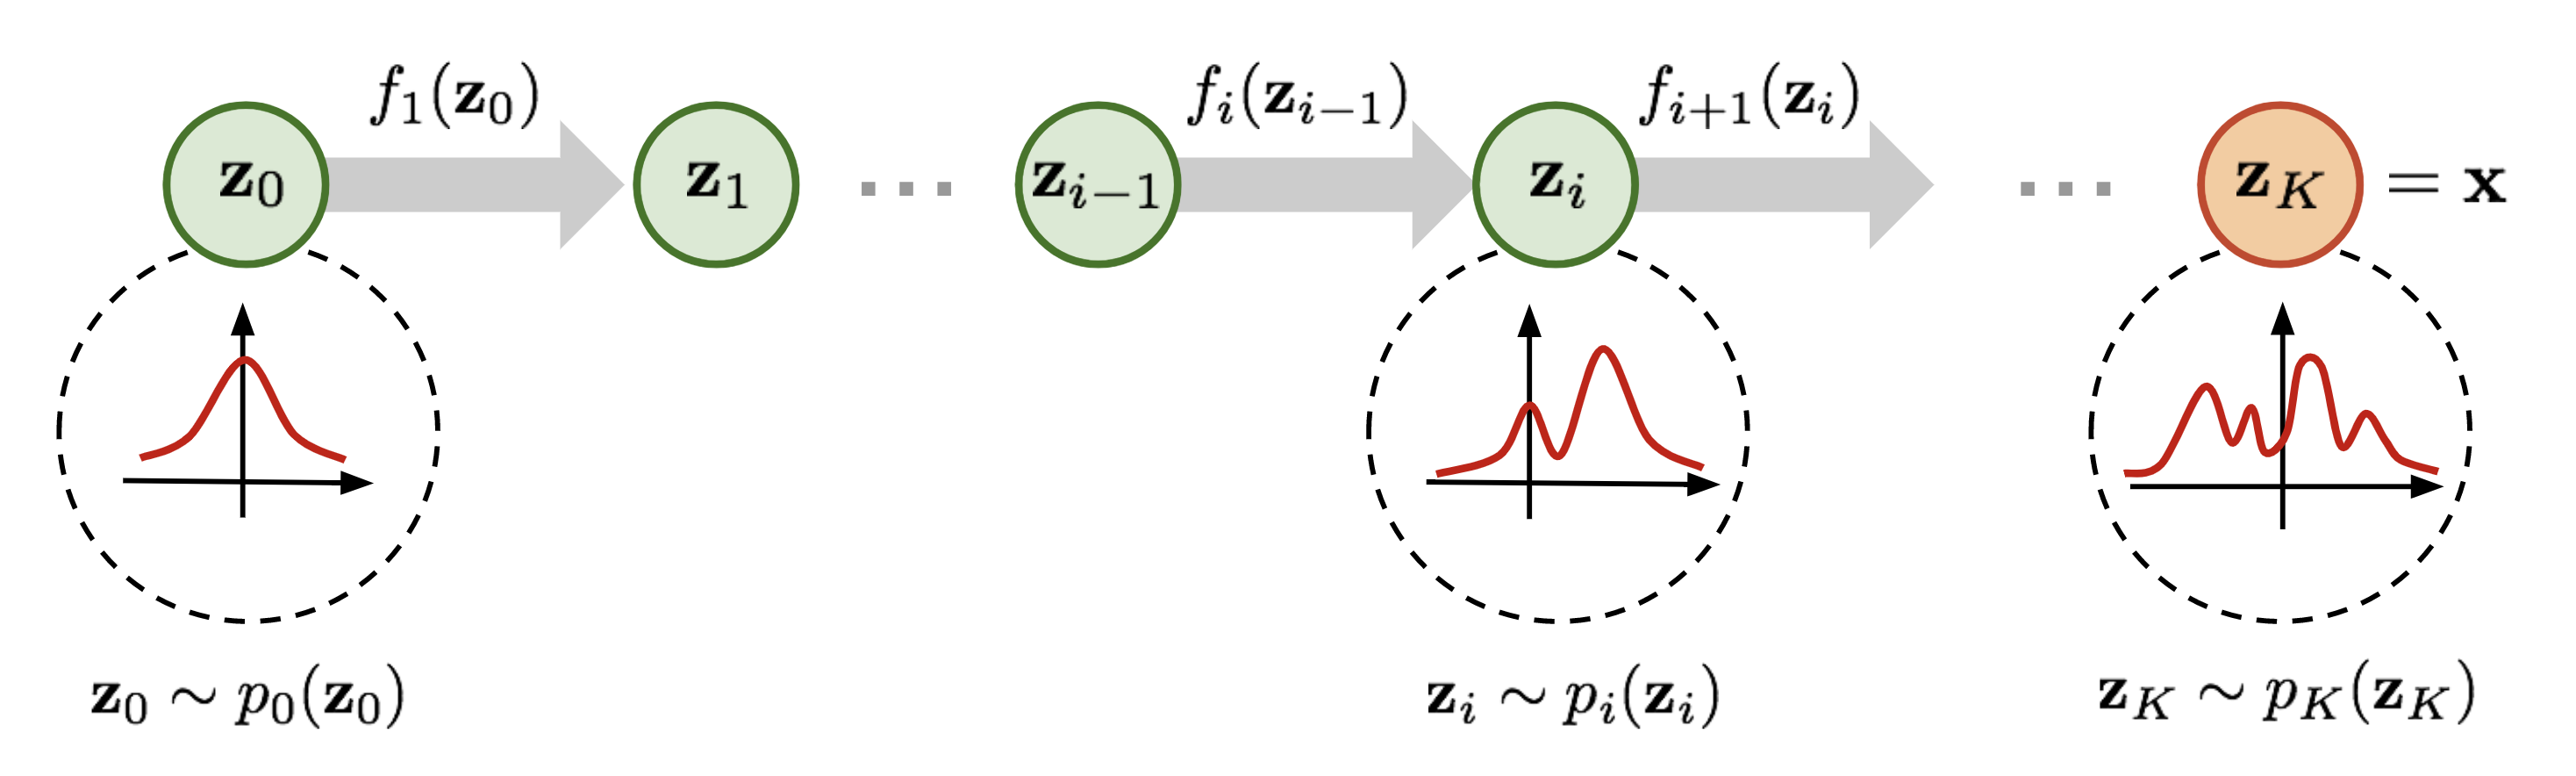
\includegraphics[width=0.95\linewidth]{figs/normalizing-flow}
	\end{figure}
	\myfootnotewithlink{https://lilianweng.github.io/lil-log/2018/10/13/flow-based-deep-generative-models.html}{https://lilianweng.github.io/lil-log/2018/10/13/flow-based-deep-generative-models.html}
\end{frame}
%=======
\begin{frame}{Normalizing flows (NF)}
	\vspace{-0.3cm}
	\[
	\log p(\bx|\btheta) = \log p(f(\bx, \btheta)) + \log |\det (\bJ_f)|
	\]
	\vspace{-0.4cm}
	\begin{block}{Definition}
		Normalizing flow is a \textit{differentiable, invertible} mapping from data $\bx$ to the noise $\bz$. 
	\end{block}
	\begin{itemize}
		\item \textbf{Normalizing} means that NF takes samples from $\pi(\bx)$ and normalizes them into samples from the density $p(\bz)$.
		\item \textbf{Flow} refers to the trajectory followed by samples from $p(\bz)$ as they are transformed by the sequence of transformations
		\[
		\bz = f_K \circ \dots \circ f_1(\bx); \quad \bx = f_1^{-1} \circ \dots \circ f_K^{-1} (\bz) = g_1 \circ \dots \circ g_K(\bz) 
		\] 
		\vspace{-0.4cm}
		\begin{block}{Log likelihood}
			\vspace{-0.4cm}
			\[
			\log p(\bx | \btheta) = \log p(f_K \circ \dots \circ f_1(\bx)) + \sum_{k=1}^K\log |\det (\bJ_{f_k})|,
			\]
			\vspace{-0.4cm} \\
			where $\bJ_{f_k} = \frac{\partial \mathbf{f}_k}{\partial \mathbf{f}_{k-1}}$.
		\end{block}
	\end{itemize}
	\textbf{Note:} Here we consider only \textbf{continuous} random variables.
\end{frame}
%=======
\begin{frame}{Normalizing flows}
	\begin{block}{Example of a 4-step NF}
		\vspace{-0.2cm}
		\begin{figure}
			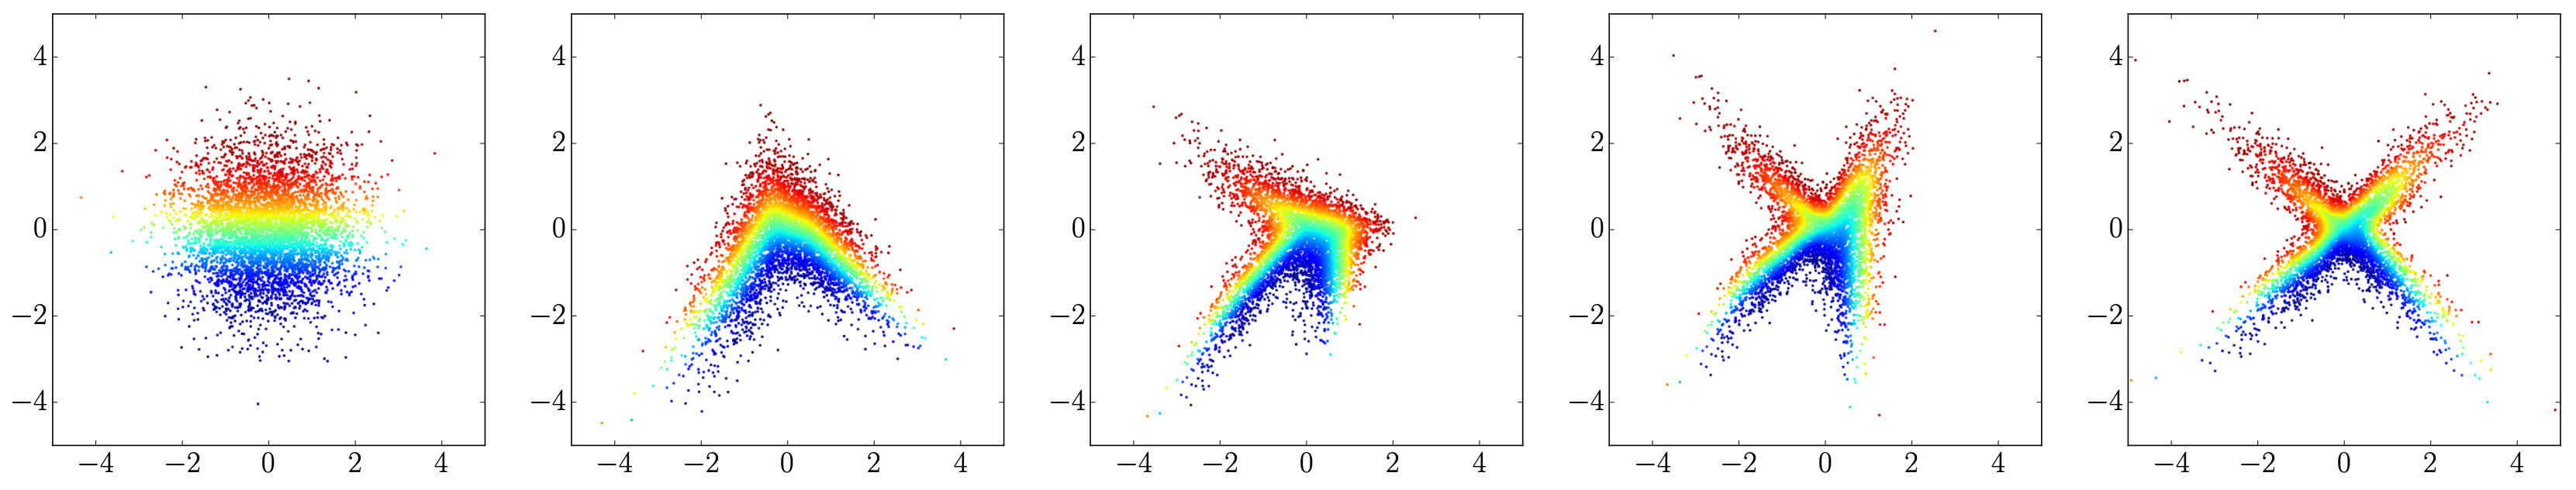
\includegraphics[width=\linewidth]{figs/flow_4_steps_example.png}
		\end{figure}
	\end{block}
	\vspace{-0.5cm}
	\begin{block}{NF log likelihood}
		\vspace{-0.3cm}
		\[
		\log p(\bx|\btheta) = \log p(f(\bx, \btheta)) + \log |\det ( \bJ_f)|
		\]
		\vspace{-0.3cm}
	\end{block}
	What is the complexity of the determinant computation?
	\begin{block}{What we need:}
		\begin{itemize}
			\item efficient computation of the Jacobian matrix $\bJ_f = \frac{\partial f(\bx, \btheta)}{\partial \bx}$;
			\item efficient inversion of $f(\bx, \btheta)$;
			\item loss function to minimize.
		\end{itemize}
	\end{block}
	\myfootnotewithlink{https://arxiv.org/abs/1912.02762}{Papamakarios G. et al. Normalizing flows for probabilistic modeling and inference, 2019} 
\end{frame}
%=======
\section{Forward and Reverse KL for NF}
%=======
\begin{frame}{Forward KL vs Reverse KL}
	\begin{block}{Forward KL $\equiv$ MLE}
		\vspace{-0.5cm}
		\begin{align*}
			KL(\pi || p) &= \int \pi (\bx) \log \frac{\pi(\bx)}{p(\bx | \btheta)} d \bx \\
			&= - \bbE_{\pi(\bx)} \log p(\bx | \btheta) + \text{const} \rightarrow \min_{\btheta}
		\end{align*}
	\end{block}
	\begin{block}{Forward KL for NF model}
	    \vspace{-0.1cm}
		\[
			\log p(\bx|\btheta) = \log p(f(\bx, \btheta)) + \log  |\det (\bJ_f)|
		\]		
		\[
			KL(\pi || p)  = - \bbE_{\pi(\bx)} \left[\log p(f(\bx, \btheta)) + \log  |\det (\bJ_f)|\right] + \text{const} 
		\]
		\vspace{-0.2cm}
		\begin{itemize}
			\item We need to be able to compute $f(\bx, \btheta)$ and its Jacobian.
			\item We need to be able to compute the density $p(\bz)$.
			\item We don’t need to think about computing the function $g(\bz, \btheta) = f^{-1}(\bz, \btheta)$ until we want to sample from the NF.
		\end{itemize}
	\end{block}
\end{frame}
%=======
\begin{frame}{Forward KL vs Reverse KL}
	\begin{block}{Reverse KL}
	  	\vspace{-0.5cm}
			\begin{align*}
				KL(p || \pi) &= \int p(\bx | \btheta) \log \frac{p(\bx | \btheta)}{\pi(\bx)} d \bx \\
				&= \bbE_{p(\bx | \btheta)} \left[{\color{violet}\log p(\bx | \btheta)} - \log \pi(\bx)\right] \rightarrow \min_{\btheta}
			\end{align*}
		\vspace{-0.7cm}
	\end{block}
	\begin{block}{Reverse KL for NF model (LOTUS trick)}
  		\vspace{-0.3cm}
		\[
			 \log p(\bx | \btheta) = \log p(\bz) +  \log  |\det (\bJ_f)| = \log p(\bz) - \log |\det (\bJ_g)| 
		\]
		\[
			KL(p || \pi)  = \bbE_{p(\bz)} \left[ {\color{violet} \log p(\bz) -  \log |\det (\bJ_g)| } - \log \pi(g(\bz, \btheta)) \right]
		\]
		\vspace{-0.3cm}
		\begin{itemize}
		\item We need to be able to compute $g(\bz, \btheta)$ and its Jacobian.
		\item We need to be able to sample from the density $p(\bz)$ (do not need to evaluate it) and to evaluate(!) $\pi(\bx)$.
		\item We don’t need to think about computing the function $f(\bx, \btheta)$.
		\end{itemize}
	\end{block}
\end{frame}
%=======
\begin{frame}{Normalizing flows KL duality}
	\begin{block}{Theorem}
		Fitting NF model $p(\bx| \btheta)$ to the target distribution $\pi(\bx)$ using forward KL (MLE) is equivalent to fitting the induced distribution $p(\bz| \btheta)$ to the base $p(\bz)$ using reverse KL:
		\vspace{-0.2cm}
		\[
			\argmin_{\btheta} KL(\pi(\bx) || p(\bx | \btheta)) = \argmin_{\btheta} KL(p(\bz | \btheta) || p(\bz)).
		\]
		\vspace{-0.7cm}
	\end{block}
	\begin{figure}
		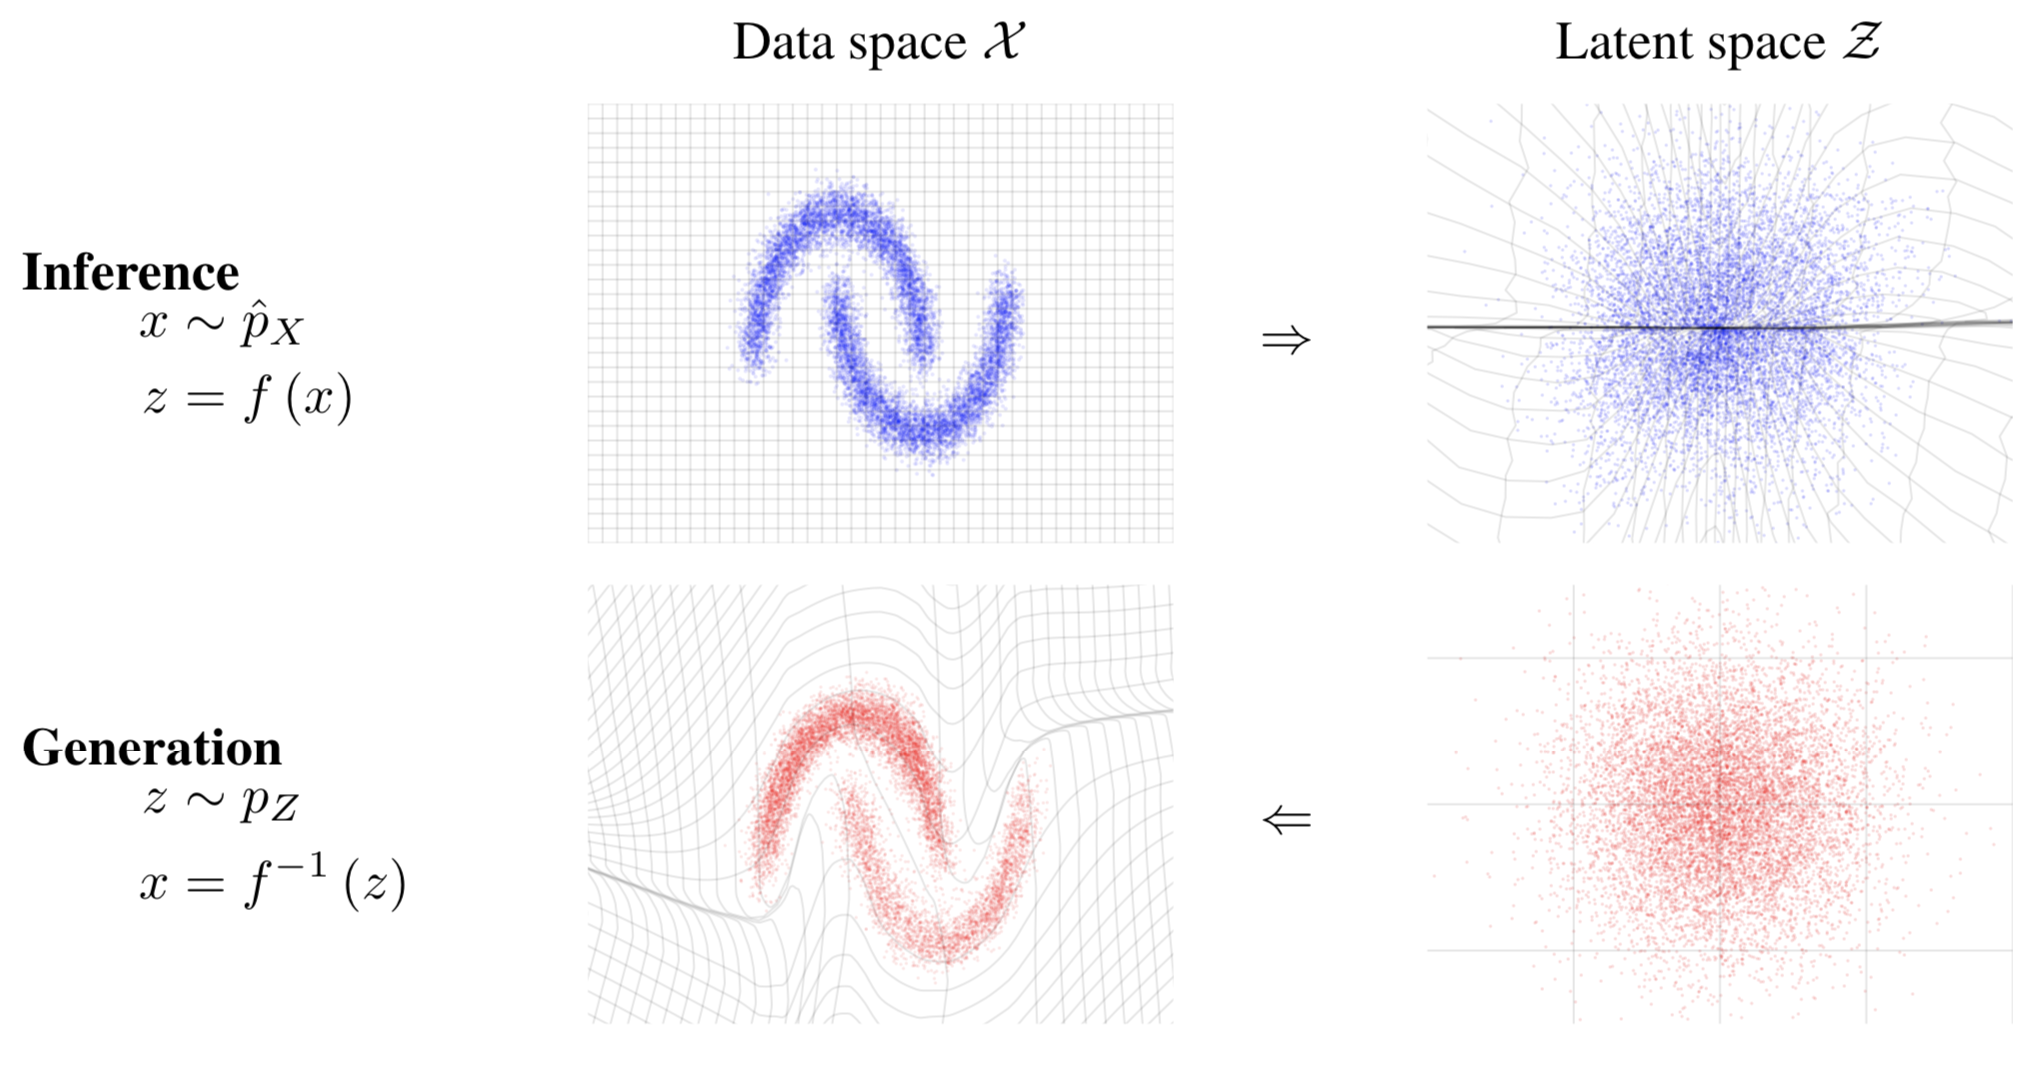
\includegraphics[width=0.85\linewidth]{figs/flows_how2}
	\end{figure}
	\myfootnotewithlink{https://arxiv.org/abs/1912.02762}{Papamakarios G. et al. Normalizing flows for probabilistic modeling and inference, 2019} 
\end{frame}
%=======
\begin{frame}{Normalizing flows KL duality}
	\begin{block}{Theorem}
		\vspace{-0.3cm}
		\[
			\argmin_{\btheta} KL(\pi(\bx) || p(\bx | \btheta)) = \argmin_{\btheta} KL(p(\bz | \btheta) || p(\bz)).
		\]
		\vspace{-0.5cm}
	\end{block}
	\begin{block}{Proof}
		\begin{itemize}
			\item $\bz \sim p(\bz)$, $\bx = g(\bz, \btheta)$, $\bx \sim p(\bx| \btheta)$;
			\item $\bx \sim \pi(\bx)$, $\bz = f(\bx, \btheta)$, $\bz \sim p(\bz | \btheta)$;
		\end{itemize}
		\vspace{-0.3cm}
		\begin{align*}
			\log p(\bz | \btheta) &= \log \pi(g(\bz, \btheta)) + \log | \det ( \bJ_g) |; \\
			\log p(\bx | \btheta) &= \log p(f(\bx, \btheta)) + \log | \det ( \bJ_f) |.
		\end{align*}
		\vspace{-0.9cm}
		\begin{multline*}
			KL\left(p(\bz | \btheta) || p(\bz) \right) = \mathbb{E}_{p(\bz | \btheta)} \bigl[ {\color{violet}\log p(\bz | \btheta)} - \log p(\bz) \bigr] = \\ 
			= \mathbb{E}_{{\color{olive}p(\bz | \btheta)}} \left[ {\color{violet}\log \pi(g(\bz, \btheta)) +  \log |\det (\bJ_g)|} - \log p(\bz) \right] = \\
			= \mathbb{E}_{{\color{olive}\pi(\bx)}} \left[ \log \pi(\bx) {\color{teal} - \log |\det (\bJ_f)| - \log p(f(\bx, \btheta))} \right] = \\
			= \mathbb{E}_{\pi(\bx)} \bigl[ \log \pi(\bx) {\color{teal} -\log p(\bx | \btheta)} \bigr] = KL (\pi(\bx) || p(\bx | \btheta)).
		\end{multline*}
	\end{block}
	\myfootnotewithlink{https://arxiv.org/abs/1705.07057}{Papamakarios G., Pavlakou T., Murray I. Masked Autoregressive Flow for Density Estimation, 2017} 
\end{frame}
%=======
\section{NF examples}
%=======
\subsection{Linear normalizing flows}
%=======
\begin{frame}{Jacobian structure}
	\begin{block}{Normalizing flows log-likelihood}
		\[
			\log p(\bx|\btheta) = \log p(f(\bx, \btheta)) + \log \left|\det \left( \frac{\partial f(\bx, \btheta)}{\partial \bx} \right) \right|
		\]
	\end{block}
	The main challenge is a determinant of the Jacobian matrix.
	\begin{block}{What is the $det(\bJ)$ in the following cases?}
		Consider a linear layer $\bz = \bW \bx$, $\bW \in \bbR^{m \times m}$.
		\begin{enumerate}
			\item Let $\bz$ be a permutation of $\bx$. 
			\item Let $z_j$ depend only on $x_j$. 
			\[
				\log \left|\det \left( \frac{\partial f(\bx, \btheta)}{\partial \bx} \right) \right| = \log \left| \prod_{j=1}^m \frac{\partial f_j(x_j, \btheta)}{\partial x_j} \right| = \sum_{j=1}^m \log \left|  \frac{\partial f_j(x_j, \btheta)}{\partial x_j} \right|.
			\]
			\item Let $z_j$ depend only on $\bx_{1:j}$ (autoregressive dependency). 
		\end{enumerate}
	\end{block}
\end{frame}
%=======
\begin{frame}{Linear normalizing flows}
	\[
		\bz = f(\bx, \btheta) = \bW \bx, \quad \bW \in \bbR^{m \times m}, \quad \btheta = \bW, \quad \bJ_f = \bW^T
	\]
	In general, we need $O(m^3)$ to invert matrix.
	\begin{block}{Invertibility}
		\begin{itemize}
			\item Diagonal matrix $O(m)$.
			\item Triangular matrix $O(m^2)$.
			\item It is impossible to parametrize all invertible matrices.
		\end{itemize}
	\end{block}
	\begin{block}{Invertible 1x1 conv}
			
		$\mathbf{W} \in \mathbb{R}^{c \times c}$ - kernel of 1x1 convolution with $c$ input and $c$ output channels.
		The computational complexity of computing or differentiating $\det (\mathbf{W})$ is $O(c^3)$.
		Cost to compute $\det (\mathbf{W})$ is $O(c^3)$. It should be invertible.
	\end{block}
	
	\myfootnotewithlink{https://arxiv.org/abs/1807.03039}{Kingma D. P., Dhariwal P. Glow: Generative Flow with Invertible 1x1 Convolutions, 2018} 
\end{frame}
%=======
\begin{frame}{Linear normalizing flows}
	\vspace{-0.5cm}
	\[
		\bz = f(\bx, \btheta) = \bW \bx, \quad \bW \in \bbR^{m \times m}, \quad \btheta = \bW, \quad \bJ_f = \bW^T
	\]
	\vspace{-0.7cm}
	\begin{block}{Matrix decompositions}
		\begin{itemize}
			\item \textbf{LU-decomposition}
			\[
				\bW = \mathbf{P} \bL \bU,
			\]
			where $\mathbf{P}$ is a permutation matrix, $\mathbf{L}$ is lower triangular with positive diagonal, $\mathbf{U}$ is upper triangular with positive diagonal.
			\item \textbf{QR-decomposition}
			\[
				\bW = \bQ \mathbf{R},
			\]
			where $\bQ$ is an orthogonal matrix, $\mathbf{R}$ is an upper triangular matrix with positive diagonal.
		\end{itemize}
	\end{block}

	Decomposition should be done only once in the beggining. Next, we fit decomposed matrices ($\bP/\bL/\bU$ or $\bQ/\bR$).

	\myfootnote{\href{https://arxiv.org/abs/1807.03039}{Kingma D. P., Dhariwal P. Glow: Generative Flow with Invertible 1x1 Convolutions, 2018}  \\
	\href{https://arxiv.org/abs/1901.11137}{Hoogeboom E., et al. Emerging convolutions for generative normalizing flows, 2019}
	}
\end{frame}
%=======
\subsection{Gaussian autoregressive NF}
%=======
\begin{frame}{Gaussian autoregressive model}
	Consider an autoregressive model
	\vspace{-0.3cm}
	{\small
		\[
		p(\bx | \btheta) = \prod_{j=1}^m p(x_j | \bx_{1:j - 1}, \btheta), \quad
		p(x_j | \bx_{1:j - 1}, \btheta) = \mathcal{N} \left(\mu_j(\bx_{1:j-1}), \sigma^2_j (\bx_{1:j-1})\right).
		\]
	}
	\vspace{-0.5cm}
	\begin{block}{Sampling: reparametrization trick}
		\vspace{-0.3cm}
		\[
		x_j = \sigma_j (\bx_{1:j-1}) \cdot z_j + \mu_j(\bx_{1:j-1}), \quad z_j \sim \mathcal{N}(0, 1).
		\]
		\vspace{-0.7cm}
	\end{block}
	\begin{block}{Inverse transform}
		\vspace{-0.3cm}
		\[
		z_j = \left(x_j - \mu_j(\bx_{1:j-1}) \right) \cdot \frac{1}{\sigma_j (\bx_{1:j-1}) }.
		\]
		\vspace{-0.4cm}
	\end{block}
	\begin{itemize}
		\item We have an \textbf{invertible} and \textbf{differentiable} transformation from $p(\bz)$ to $p(\bx | \btheta)$.
		\item It is an autoregressive (AR) NF with the base distribution $p(\bz) = \cN(0, 1)$!
		\item Jacobian of such transformation is triangular!
	\end{itemize}
	\myfootnotewithlink{https://arxiv.org/abs/1606.04934}{Kingma D. P. et al. Improving Variational Inference with Inverse Autoregressive Flow, 2016} 
\end{frame}
%=======
\begin{frame}{Gaussian autoregressive NF}
	\vspace{-0.2cm}
	\begin{align*}
		\bx &= g(\bz, \btheta) \quad \Rightarrow \quad {\color{violet} x_j} = \sigma_j ({\color{violet} \bx_{1:j-1}}) \cdot {\color{teal} z_j} + \mu_j({\color{violet} \bx_{1:j-1}}). \\
		\bz &= f(\bx, \btheta) \quad \Rightarrow \quad {\color{teal} z_j} = \left({\color{violet}x_j} - \mu_j({\color{violet}\bx_{1:j-1}}) \right) \cdot \frac{1}{ \sigma_j ({\color{violet}\bx_{1:j-1}})}.
	\end{align*}
	Generation function $g(\bz, \btheta)$ is \textbf{sequential}. \\ Inference function $f(\bx, \btheta)$ is \textbf{not sequential}.

	\begin{block}{Forward KL for NF}
		\vspace{-0.5cm}
		\[
			KL(\pi || p)  = - \bbE_{\pi(\bx)} \left[\log p(f(\bx, \btheta)) + \log  |\det (\bJ_f)|\right] + \text{const} 
		\]
		\vspace{-0.5cm}
		\begin{itemize}
			\item We need to be able to compute $f(\bx, \btheta)$ and its Jacobian.
			\item We need to be able to compute the density $p(\bz)$.
			\item We don’t need to think about computing the function $g(\bz, \btheta) = f^{-1}(\bz, \btheta)$ until we want to sample from the model.
		\end{itemize}
	\end{block}
	\myfootnotewithlink{https://arxiv.org/abs/1705.07057}{Papamakarios G., Pavlakou T., Murray I. Masked Autoregressive Flow for Density Estimation, 2017} 
\end{frame}
%=======
\begin{frame}{Summary}
	\begin{itemize}
		\item Change of variable theorem allows to get the density function of the random variable under the invertible transformation.
		\vfill
		\item Normalizing flows transform a simple base distribution to a complex one via a sequence of invertible transformations with tractable Jacobian.
		\vfill
		\item Normalizing flows have a tractable likelihood that is given by the change of variable theorem.
		\vfill
		\item We fit normalizing flows using forward or reverse KL minimization. 
		\vfill 
		\item Linear NF try to parametrize set of invertible matrices via matrix decompositions.
		\vfill
		\item Gaussian autoregressive NF is an autoregressive model with triangular Jacobian. It has fast inference function and slow generation function. Forward KL is a natural loss function.
	\end{itemize}
\end{frame}
\end{document} 